

\chapter{Normalization}
\label{ch:normalization}



There seems to be a lot of ambiguity when it comes to data normalization. First of all, what what do we mean when we say normalization? There are actually many different types of normalization! For example, there are often no clear answers given to questions such as when should I normalize my data? Should I combine data from different sources? Do I need to transform my data? We present here some guidelines for such situations, but stress that the reason such ambiguity exists, is because the answer usually comes down to making a judgment call. For example, you need to weigh up the options in terms of asking what assumptions are being made or being violated by normalizing the data.

\section{Normalization by standardization}

First of all, let's discuss the different types of normalization. Many people would think of standardization; whereby we subtract the mean and divide by the standard deviation to obtain data with mean zero and a standard deviation of 1. But even standardization raises questions: for example, what are we subtracting the mean of? Do we simply take the mean of all of the numbers in our dataset, and subtract this global mean from each number? Do do this process for each variable separately, so that each variable has zero mean and unit variance? Why not for each observation instead? Further, what if we had split our data into a training and test set; do we standardize these datasets separately after the split or together, before the split?


\section{Normalization for comparison}

There are also other kinds of normalization. For example, normalization of data from different sources to improve comparability. For example, suppose we obtained fMRI data from 10 different people. Are the responses from each person comparable? Why or why not? The data from different people may not be comparable for many reasons: for example, each run of the fMRI experiment may have slightly different calibration, each persons brain has slightly different shapes and must be transformed differently to fit the image template. 

\section{Normalization by transformation}

Perhaps instead it is a transformation that comes to mind. Some may interpret normalization to be a process that makes the data look more normally distributed, perhaps by taking the log of a variable. Recall that many theoretical results rest on the assumption that the data is normally distributed. Thus perhaps we can attempt to reduce the amount by which we violate such assumptions by making our data appear more Gaussian. When might a log-transform work well? 

\begin{enumerate}
\item If we have fit a linear model to some response which is actually multiplicatively related to the predictors, then obviously the model is not going to be an accurate representation of the relationships between the variables. Taking a log-transformation of the response however, means that we can capture this relationship using an additive linear model since if $y = a \times b$ then $\log y = \log a + \log b$. 
\item If we are using a procedure that assumes Gaussianity (which, by the way, a standard linear model does not!), and we have a skewed distribution, then taking a log-transform can downplay the skewness generating a more normal distribution:
\end{enumerate}


%http://www.geo.mtu.edu/volcanoes/vc_web/background/graphics/log.jpg
\begin{figure}[H]
\begin{center}
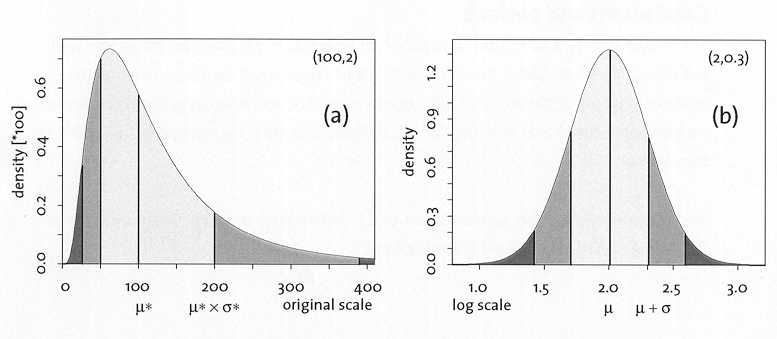
\includegraphics[scale=0.7]{log.jpg}
\end{center}
\caption{A log-transformation of a skewed distribution.}
\label{fig:log}
\end{figure}


What about other transformations? Another popular transformation is the square-root transformation. The square-root transformation is also commonly used to make data closer approximate a normal distribution. Both the log and the square-root transformations "squeeze" the data towards the mean. In fact, the two functions are notably similar:

%http://people.uncw.edu/norris/133/Onotation/images/SomeFunctions3.gif
\begin{figure}[H]
\begin{center}
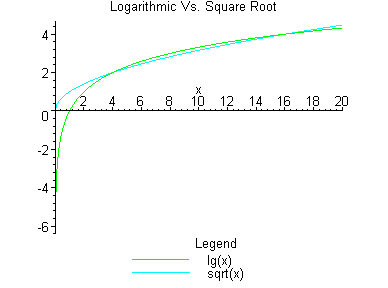
\includegraphics[scale=0.7]{log_sqrt.png}
\end{center}
\caption{The logarithmic transformation versus the square-root transformation}
\label{fig:log_sqrt}
\end{figure}

A more general transformation is the Box-Cox transformation.



Note that it is a common misconception that standard linear models assume that the data is normal. This is not the case. We will discuss in later sections that such models do not assume any distribution, but some people impose normality assumptions on the \emph{error} terms. The primary reason that it is so common to transform the data to increase normality prior to fitting a linear model is because the linear model tends to work a lot better when we have normally distributed data, although normality is not an explicit assumption of OLS.





\subsection*{What happens when we transform? Kernel density estimation example}

Suppose that we wanted to use kernel density estimation and had selected a good bandwidth. What bandwidth should we choose if we want to transform the data but retain the same amount of detail? Would it be the same? Do we just apply the same transformation to the bandwidth?

To illustrate, let's consider the model size example (whereby we were using CV to select the regularization parameter for the lasso model) which recorded how many variables were selected in the model for each parameter \textcolor{red}{or something like that...}. Suppose that we originally had a bandwidth of 3 (the left-hand plot), but we wanted to take a log-transformation of the data. The right-hand plot shows what would happen if we also log-transformed the bandwidth, so that we used a bandwidth of $\log(3)$:


\begin{figure}[H]
\begin{center}
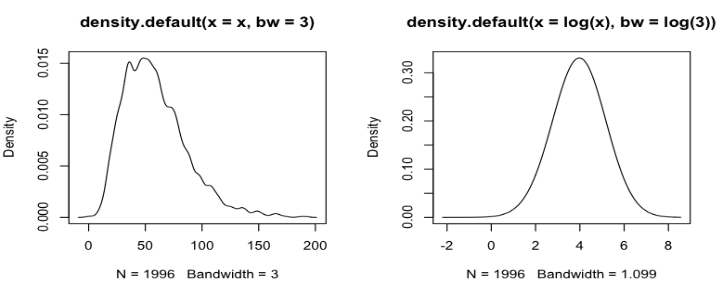
\includegraphics[scale=0.5]{log-transform-kernel.png}
\end{center}
\caption{The effect of a logarithmic transformation on the bandwidth of a kernel function}
\label{fig:log_kernel}
\end{figure}


Clearly a lot of the variance has been lost, and we have obtained a much smoother density estimate. The right-hand plot with the log-transformed bandwidth is much less variable. \textcolor{red}{Show also an example of what happens if we just don't transform the bandwidth? i.e. (x = log(x), bw = 3)}. 

How could we instead do a meaningful transformation. To answer this question, we turn to the \textbf{delta-method}. The delta method tells us how the variance of a random variable changes after a transformation, and it arises from the Taylor expansion of $g(X)$ (the details of which are shown in the appendix). In particular, suppose we have a transformation $g$ (we might have $g(x) = \log(x)$ or $g(x) = \sqrt(x)$). Suppose $X$ is a random variable such that $\mu_X = E(X)$, then the variance of the transformed random variable, $g(X)$, can be written as

$$Var(g(X)) \approx \left(g^\prime(\mu_X)\right)^2 Var(X) = Var(g^\prime(\mu_X) X)$$

For example, if $g(t) = \log (t)$, then $g^\prime(t) = \frac1t$, similarly, if $g(t) = \sqrt{t}$ then $g^\prime(t) = \frac{1}{2\sqrt{t}}$ 

This tells us that our new bandwidth should be scaled by $g^\prime(\mu_X)$. Thus, since the mean of the CV model size dataset is $\mu_X \approx 58.8$, when we take the log-transformation, we take the transformed bandwidth to be

$$h_{log} = \frac{h}{58.8}$$

and when we take the square-root transformation, we use

$$h_{square-root} = \frac{h}{2\sqrt{58.8}}$$

where $h=3$ is our original bandwidth.

Using these transformations, we obtain kernel density estimates that have the same level of variability as the original untransformed plot. In addition, the square-root transformation has also normalized the data quite nicely.

\begin{figure}[H]
\begin{center}
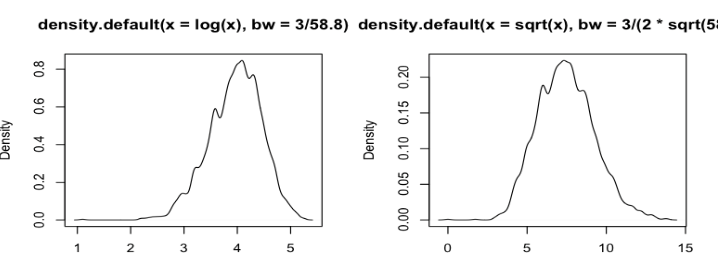
\includegraphics[scale=0.5]{log-transform-kernel2.png}
\end{center}
\caption{The effect of a logarithmic transformation on the bandwidth of a kernel function}
\label{fig:log_kernel2}
\end{figure}

Does this always work? In short: no it won't. In particular, if our estimate of the mean is extremely variable (a large standard deviation), or if the bulk of the data is far from the mean (as is the case for bimodal distributions), then the linear expansion given by the delta-method will be a poor approximation.



\section{Normalization in real life}

Often, normalization removes a lot of the natural dependence structures that exist within the data. Further, if the variables had meaningful units such that interpretations after scaling become less transparent, we might be enticed to leave the data alone.




So with this in mind, why would we ever want to normalize our data? Let's begin by giving some real-life examples.


It is probably not a reasonable assumption that the voxels are independent to one another, right? But as soon as we don't have independence, some of the most useful models are no longer applicable. Often we assume independence because we don't know how to model the dependence. Most assumptions that we make on our data are assumptions of convenience. Thus the question becomes, if the assumptions of our model are a little bit wrong, how much of an impact will this have on our conclusions drawn from these models? 


Further, what assumptions would we be making by combining the voxel responses from different sessions different people (or even from the same person)? We collected the voxel responses from a number of people, but we chose to analyze them separately. Why? The primary reason is that to combine the data from different people would mean that we had to ensure that the data were normalized (and thus comparable). But how could we do this? In a lot of applied problems, people simply collate their data from different sources together without considering whether this action makes sense.

The issue of normalization is also extremely prevalent in areas of bioinformatics, whereby each run of an experiment has different sources of bias. When the microarray technology first appeared, it was the first time scientists were able to actually look at the expression levels of multiple genes at once. The process of microarray data generation is very physical; someone must fluorescent tag the genes with chemicals and wash away the genetic materials that are not of interest. The data requires so much pre-processing and can be so noisy. \textcolor{red}{Perhaps talk about normalization in terms of microarray data more}. 

\begin{itemize}
\item {\bf Word/phrase counts from different documents}
\item {\bf Width of the stripe to normalize the gap size in fruitfly project (ongoing)}. We performed a log-transform for the gap data to make it more normal.
\end{itemize}

\begin{figure}[H]
\begin{center}
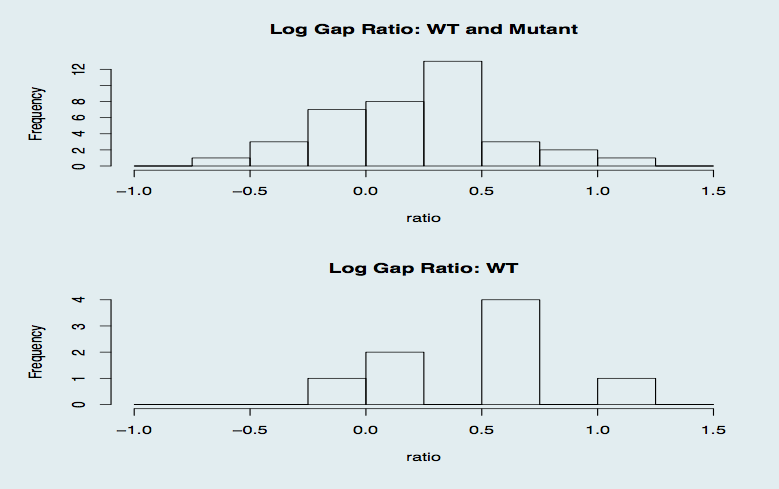
\includegraphics[scale=0.5]{gap-log.png}
\end{center}
\caption{Taking a log-transformation of the gap data}
\label{fig:log_kernel2}
\end{figure}




\section{Appendix: The delta-method}

Suppose $X$ is a random variable, where $EX = \mu_X$. A first-order Taylor expansion of $g(X)$ about $\mu_X$ is given by

$$g(X) \approx g(\mu_X) + g^\prime(\mu_X)(X - \mu_X)$$

Thus
$$E(g(X)) \approx g(\mu_X)$$

and

$$Var(g(X)) \approx g^\prime(\mu_X)Var(X)$$


To apply the delta method in reality, we don't know $\mu_X$, so we estimate it by the sample mean. In particular, this method will work well when the sample mean is close to the true mean, which will often be the case if the spread is not huge; if the variability of our estimate of the mean is small relative to the size of the mean. 

Consider, however, the example where the distribution of $X$ is bimodal. In this case, this will yield a bad approximation; since the bulk of the data will be far from this estimate of the mean.